\documentclass[final,hyperref={pdfpagelabels=false}]{beamer}

\usepackage[orientation=portrait,size=a0,scale=0.82]{beamerposter}

\usetheme{HorGagSawPos} % beamerthemeHorGagSawPos
\usepackage[english]{babel} % English language/hyphenation

\usepackage{amsmath,amsthm,amssymb,latexsym} % For including math equations, theorems, symbols, etc

\usepackage{multirow} % multirow in tables
\usepackage{hhline} 

% to work with tabular
\usepackage{xcolor,colortbl}

% align in arrays
\usepackage{array}
\newcolumntype{L}[1]{>{\raggedright\let\newline\\\arraybackslash\hspace{0pt}}m{#1}}
\newcolumntype{C}[1]{>{\centering\let\newline\\\arraybackslash\hspace{0pt}}m{#1}}
\newcolumntype{R}[1]{>{\raggedleft\let\newline\\\arraybackslash\hspace{0pt}}m{#1}}

%\usepackage{times}\usefonttheme{professionalfonts}  % Uncomment to use Times as the main font
%\usefonttheme[onlymath]{serif} % Uncomment to use a Serif font within math environments

%\boldmath % Use bold for everything within the math environment

\usepackage[skins,theorems]{tcolorbox}
\tcbset{highlight math style={enhanced,
  colframe=red,colback=white,arc=0pt,boxrule=1pt}}

\usepackage{booktabs} % Top and bottom rules for tables

\graphicspath{{figures/}} % Location of the graphics files

\usecaptiontemplate{\small\structure{\insertcaptionname~\insertcaptionnumber: }\insertcaption} % A fix for figure numbering

%----------------------------------------------------------------------------------------
%	TITLE SECTION 
%----------------------------------------------------------------------------------------

\title{\huge Towards the HPC-inference of causality networks\\[0.8ex] from multiscale economical data} % Poster title

\author{\hfill\Large Illia~Horenko$^{ 1}$, Patrick~Gagliardini$^{ 1}$, William~Sawyer$^{ 2}$, Luk\'{a}\v{s} Posp\'{i}\v{s}il$^{ 1}$}

\institute{\large \hfill  $^{1}$ Universit\`a della Svizzera Italiana (USI Lugano),
				  $^{2}$ Swiss National Supercomputing Centre (CSCS/ETH Zurich),\\[1ex]
			\hfill {\tt \large [illia.horenko@usi.ch, patrick.gagliardini@usi.ch, william.sawyer@cscs.ch, lukas.pospisil@usi.ch]} }

%----------------------------------------------------------------------------------------

\begin{document}

\addtobeamertemplate{block end}{}{\vspace*{2ex}} % White space under blocks

\begin{frame}[t] % The whole poster is enclosed in one beamer frame


\begin{columns}[t] % The whole poster consists of two major columns, each of which can be subdivided further with another \begin{columns} block - the [t] argument aligns each column's content to the top

\begin{column}{.01\textwidth}\end{column} % Empty spacer column

\begin{column}{.48\textwidth} % The first column

%----------------------------------------------------------------------------------------
%	Focus of the project
%----------------------------------------------------------------------------------------

\begin{block}{Focus of the project}

Analysis of large amounts of economical data and data-driven inference of causality relations between different
components of economical systems  is one of the central problems in modern computational finance and economics. 
The task of proper mathematical description and adequate causality understanding for the economical data is hampered
by the multiscale nature of the underlying processes, resulting from the presence of different temporal and spatial, i.e. regional, sectorial and global, scales.

\vskip2ex

\noindent Important challenges are: 
\begin{itemize}
 \item[(i)] an investigation of the mutual causality influences of different economic observables and their spatial (e.g., regional) and temporal (e.g., associated with the business cycle) evolution, 
 \item[(ii)] identification of the most important exogenous impact factors that play a role in their dynamics, 
 \item[(iii)] proper mathematical and statistical description of the influences coming from the unresolved/latent scales and factors. 
\end{itemize}
The solution of these problems can be enhanced by  analysis of  a causality network inferred from the data.  This network is a directed weighted graph with edges representing the causality relations between the  different economical variables, exogenous factors, etc. (situated at the vertices of this causality graph). Analysis of this graph would allow to understand the most important features of the underlying complex economical system.

\vskip2ex

{\color{blue}
\noindent Milestone questions about the targeted economical data:
\begin{enumerate}
  \item {\color{blue}Is there a causality relation between different sectors of the economy with respect to the credit risk migrations?'}
  \item {\color{blue}What is the most effective implementation of the multiscale causality inference framework in the embarassingly-parallel case?}
  \item {\color{blue}Are there any statistically-significant causality impacts from other sectors on the companies inside of the `Banking and Finance' sector?}
  \item {\color{blue}Among all of the considered alternatives and platforms, what is the most scalable implementation for multiscale causality inference?}
\end{enumerate}
}
%\vskip2ex
\end{block}

%----------------------------------------------------------------------------------------
%	Understanding Causality
%----------------------------------------------------------------------------------------
            
\begin{block}{Non-stationary modelling}

We suppose that unknown parameters of the model $\theta$ are changing in time
\begin{displaymath}
 \theta^{*}(t) = \arg \min\limits_{\theta(t)} \int\limits_{0}^{T} g(x(t), \theta(t)) ~dt
  ~~ \approx ~~ 
  \arg \min\limits_{\theta(t)} \sum\limits_{t=0}^{T} g(x_t, \theta(t)),
\end{displaymath}
where $g(x(t),\theta)$ represents local model error (or equivalently negative value of maximum likelihood function), for example
\begin{displaymath}
 \begin{array}{c}
 g(x(t),\theta(t)) = \left\Vert x(t) - \theta(t) \right\Vert^2 ~~~\textrm{(K-means model)}, ~~~~~
 g(x(t),\theta(t)) = \left\Vert x(t) - \left(\sum\limits_{p=0}^{m} \alpha_{p}(t) t^p \right) \right\Vert^2 ~~~ \textrm{(polynomial regression)}, \\[2em]
 g(x(t),\theta(t)) = \left\Vert x(t) - \left(\mu(t) +\sum_{i=0}^p A_{i}(t) x(t-i\tau) + \sum_{j=0}^q B_{j}(t) y^{t-j\tau} \right) \right\Vert^2  ~~~\textrm{(autoregressive models)}.
 \end{array}
\end{displaymath} 
\end{block}

\begin{block}{Assumptions}
\begin{itemize}

\begin{columns}[T]
\begin{column}{0.02\linewidth}\end{column}
\begin{column}{0.94\linewidth}
\item[1.)] $\forall t ~\textrm{in $k$-th cluster}: ~\theta(t) = \theta_k$  (i.e. $\theta$ is constant on cluster)
\begin{displaymath}
 [\Theta^{*}, \Gamma^{*}(t) ] = \arg \min\limits_{\Theta,\Gamma} \int\limits_{0}^{T} \sum\limits_{k=1}^K \gamma_k(t) \cdot g(x(t), \theta_k) ~dt
  ~~ \approx ~~ 
  \arg \min\limits_{\Theta,\Gamma} \sum\limits_{t=0}^{T} \sum\limits_{k=1}^{K} \gamma_{k,t} \cdot g(x_t, \theta_k)
\end{displaymath}
where each cluster is determined by 
\end{column}	
\begin{column}{0.02\linewidth}\end{column}
\end{columns}
\vskip1ex
\begin{displaymath}
 \tcbhighmath[fuzzy halo=1mm with blue!50!white,arc=2pt,
 boxrule=0pt,frame hidden]{ 
 \begin{array}{rcl}
  \theta_k &~~~& \textrm{vector of cluster stationary model parameters (depends on used model)}, \\[1em]
  \gamma_k & & \textrm{model indicator function} ~~ \gamma_k(t) \in \lbrace 0,1 \rbrace, ~~ \gamma_k(t) = \left\lbrace
  \begin{array}{ll}
   1~ & \textrm{if $k$-th cluster is active in $t$} \\
   0~ & \textrm{if $k$-th cluster is inactive in $t$}
  \end{array}
 \right. ~\textrm{and exactly one cluster is active in $t$}
 \end{array}
 }
\end{displaymath}
\vskip3ex
\end{itemize}
\begin{columns}[T]
\begin{column}{0.02\linewidth}\end{column}
\begin{column}{0.64\linewidth}
\begin{itemize}
 \item[2.)] continuous real-valued functions $\gamma_k(t) \in [0,1]$
 \begin{equation}
  \label{eq:loglik_lb_con}
  0 \leq \gamma_k(t) \leq 1, ~~
  \forall t: \sum\limits_{k=1}^K \gamma_k(t) = 1
 \end{equation}
\vskip3ex
 \item[3.)] smooth $\gamma_k(t)$ $~\Rightarrow~$ regularisation, $\Vert \gamma \Vert_{H1} \leq \Vert x \Vert_{H1}$
 \begin{displaymath}
 \int\limits_{0}^{T} \sum\limits_{k=1}^K \gamma_k(t) \cdot g(x(t), \theta_k) ~dt {\color{red} + \varepsilon^2 \sum\limits_{k=1}^K \int\limits_0^T (\partial_t \gamma_k(t))^2 dt}
 ~~~~~~~~~~~~~~~~~~~~~~~~~~~~~~~~~~
 \end{displaymath}
 \begin{displaymath}
  \textrm{(using FEM hat functions)}~~~~~~~~ \approx ~~ 
  \sum\limits_{t=0}^{T} \sum\limits_{k=1}^{K} \gamma_{k,t} \cdot g(x_t, \theta_k)
    {\color{red} + \varepsilon^2 \sum\limits_{k=1}^K \sum\limits_{t=0}^{T-1} (\gamma_{k,t+1} - \gamma_{k,t})^2}
 \end{displaymath}
 \end{itemize}
\end{column}	
\begin{column}{0.30\linewidth}
	\begin{figure}[H]
		\begin{center}
			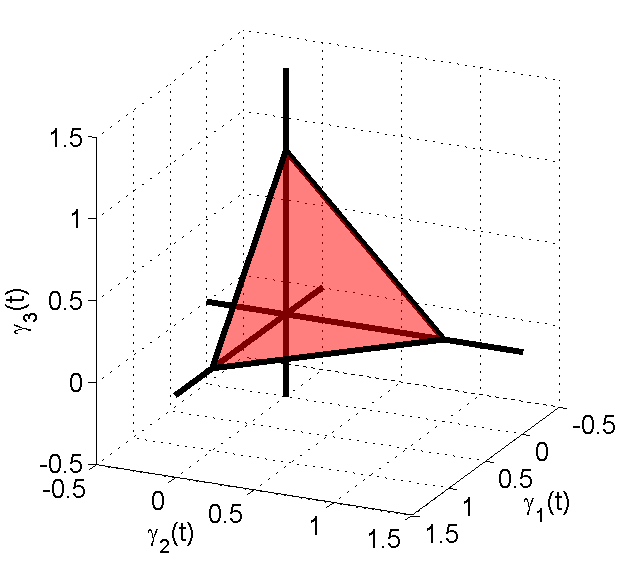
\includegraphics[width=0.9\linewidth, angle=0, clip = true]{figures/simplex.png}
		\end{center}
	\end{figure}
\end{column}	
\begin{column}{0.02\linewidth}\end{column}
\end{columns}



\end{block}



%----------------------------------------------------------------------------------------
%	High Performance Computing Implementation
%----------------------------------------------------------------------------------------

\begin{block}{Solving the problem}

The optimisation problem is given by
\begin{equation}
\label{eq:general}
 [\Theta^{*}, \Gamma^{*} ] = 
  \arg \min\limits_{\Theta,\Gamma} \sum\limits_{t=0}^{T} \sum\limits_{k=1}^{K} \gamma_{k,t} \cdot g(x_t, \theta_k)
  + \varepsilon^2 \sum\limits_{k=1}^K \sum\limits_{t=0}^{T-1} (\gamma_{k,t+1} - \gamma_{k,t})^2 ~~~
 ~~ \textrm{s.t.} ~~ 0 \leq \gamma_{k,t} \leq 1, ~
 \forall t: \sum\limits_{k=1}^K \gamma_{k,t} = 1.
\end{equation}
This nonconvex problem \eqref{eq:general} could be solved iteratively as a sequence of solution of two optimisation problems, see Algorithm \ref{alg:outer}.

\begin{columns}[T]
\begin{column}{0.02\linewidth}\end{column}

\begin{column}{0.45\linewidth}
	\begin{center}
	\begin{table}[h!]
	\renewcommand{\tablename}{Algorithm}
	\fbox{\it
	\begin{tabular}{p{0.95\linewidth}}
	\medskip
	\hspace*{0.6CM}set feasible initial approximation $\Gamma_{0}$\\
	\medskip
	\hspace*{0.6CM}{\textbf{while}} $\Vert L(\Gamma_{it},\Theta_{it}) - L(\Gamma_{it-1},\Theta_{it-1}) \Vert \geq \varepsilon$\\[2em]
	\hspace*{1.2CM} solve $\Theta_{it} = \arg \min\limits_{\Theta} L(\Theta, \Gamma_{it-1})$ $~~~$ (with fixed $\Gamma_{it-1}$) \\[2em]
	\hspace*{1.2CM} solve $\Gamma_{it} = \arg \min\limits_{\Gamma} L(\Theta_{it}, \Gamma)$ $~~~$ (with fixed $\Theta_{it}$) \\[2em]
	\hspace*{1.2CM} $it = it + 1$ \\
	\hspace*{0.6CM}{\textbf{endwhile}} \\
	\medskip
	\end{tabular}
	}
	\caption{\label{alg:outer} \bf Outer algorithm.}
	\end{table}
	\end{center}

	\vskip1.5ex
	
	\begin{equation}
	\label{eq:qpp}
	\tcbhighmath[fuzzy halo=1mm with blue!50!white,arc=2pt,
	boxrule=0pt,frame hidden]{ 
	\begin{array}{c}
		\Gamma_{it} = \arg\min \frac{1}{2} \gamma^T H \gamma + g^T \gamma \\[1ex]
		\textrm{subject to} ~~~ \forall t: \sum\limits_{k=1}^{K} \gamma_{k}^t = 1, \gamma \geq 0. \\[5ex]
		H \in \mathbb{R}^{K \cdot T,K \cdot T}, ~~g, \gamma \in \mathbb{R}^{K \cdot T}
	\end{array}
	}
	\end{equation}
	
	\vskip3.5ex
	
	\begin{equation}
	 \label{eq:aic}
	 AIC(L,\Theta,K) = - 2 \ln L + 2 (\textrm{sizeof}(\Theta) + K)
	\end{equation}
\end{column}	

\begin{column}{0.49\linewidth}
	\begin{center}
	\begin{table}[h!]
	\renewcommand{\tablename}{Algorithm}
	\fbox{\it
	\begin{tabular}{p{1.0\linewidth}}
Given cost function $f: \mathbb{R}^n \rightarrow \mathbb{R}$, 
initial approximation $x^{0} \in \Omega$, 
projection onto feasible set $P_{\Omega}(x)$,
parameters $m \in \mathbb{N}, \gamma \in (0,1)$, 
safeguarding parameters $\sigma_1, \sigma_2\in \mathbb{R}: 0 < \sigma_1 < \sigma_2 < 1$,
precision $\varepsilon > 0$, and
initial step-size $\alpha_0 > 0$. \medskip \\
\hspace*{0.6CM} $k := 0$\\
\hspace*{0.6CM} $g^0 := Ax^0 - b$\\
\hspace*{0.6CM} $f^0 := 1/2 \langle g^0 - b, x^0 \rangle$ \medskip \\
%\hspace*{1.2CM} $\alpha_0 := \langle g^0, g^0 \rangle / \langle Ag^0, g^0 \rangle$\\
\hspace*{0.6CM} {\rm\textbf{for}} $k = 0,1,\dots$\\
\hspace*{1.2CM} $d^k := P_{\Omega}(x^k - \alpha_k g^k) - x^k$  \medskip\\
\hspace*{1.2CM} compute matrix-vector multiplication $A d^k$ \\
\hspace*{1.2CM} compute multiple dot-product $\langle d^k, \lbrace d^k, Ad^k, g^k \rbrace \rangle$ \medskip \\
\hspace*{1.2CM} if $\sqrt{\langle d^k, d^k \rangle} \leq \varepsilon$ then stop.\medskip\\
\hspace*{1.2CM} $f_{\max} := \max \lbrace f(x^{k-j}): 0 \leq j \leq \min \lbrace k,m-1 \rbrace \rbrace$ \\
\hspace*{1.2CM} $\xi := (f_{\max} - f^k) / \langle d^k, A d^k \rangle$ \\
\hspace*{1.2CM} $\bar{\beta} := - \langle g^k, d^k \rangle / \langle d^k, A d^k \rangle$ \\ 
\hspace*{1.2CM} $\hat{\beta} := \gamma \bar{\beta} + \sqrt{\gamma^2\bar{\beta}^2 + 2 \xi}$ \\ 
\hspace*{1.2CM} choose $\beta_k \in \langle \sigma_1, \min \lbrace \sigma_2, \hat{\beta} \rbrace \rangle$ \medskip \\ 
\hspace*{1.2CM} $x^{k+1} := x^k + \beta_k d^k$\\
\hspace*{1.2CM} $g^{k+1} := g^k + \beta_k A d^k$\\
\hspace*{1.2CM} $f^{k+1} := f^k + \beta_k \langle d^k, g^k \rangle + \frac{1}{2} \beta_k^2 \langle d^k, Ad^k \rangle$  \medskip\\
\hspace*{1.2CM} $\alpha_{k+1} := \langle d^k, d^k \rangle / \langle d^k, Ad^k \rangle$ \medskip\\
\hspace*{1.2CM} $k := k + 1$ \\
\hspace*{0.6CM} {\rm\textbf{endwhile}} \\
\medskip
Return approximation of solution $x^{k}$.
	\end{tabular}
	}
	\caption{\label{alg:spg_qp} \bf Spectral projected gradient method for QP.}
	\end{table}
	\end{center}
\end{column}	
\begin{column}{0.02\linewidth}\end{column}
\end{columns}
\vskip3ex
Please notice that the second problem in Algorithm \ref{alg:outer} (i.e. $\Gamma$-problem) is independent of selected model.
The model indicator functions $\Gamma$ are represented by vector of dimension $K \cdot T$
and they have to fullfill conditions \eqref{eq:loglik_lb_con}. The obtained optimisation problem is Quadratic Programming problem
with SPS Hessian matrix and feasible set defined by simplex (3). Solving this problem is the most time-consuming operation.
\vskip2ex
In our library, we are using a Spectral Projected Gradient method (see Martinez et al. \cite{spg}) simplified for QP problems (see Algorithm \ref{alg:spg_qp}) developed by Pospisil \cite{pospisil_phd}.
The algorithm is based on the solving the sequence of projection problems and since the feasible set is described by separable simplex constraints (of dimension $K$),
this system extends the granularity of the solution process and it is suitable for GPU.
\vskip2ex
Since the number of clusters $K$ is unknown, the optimisation problem \eqref{eq:general}
with different choice of these parameters has to be solved. Also different choise of initial $\Gamma_0$ leads to different results.
These problems are completely independent and leads to the straightforward parellelisation. In the end of solution process, the solution with the lowest AIC number \eqref{eq:aic}
is chosen as a solution of the original problem. \newline
\end{block}

%----------------------------------------------------------------------------------------
%	Acknowledgements
%----------------------------------------------------------------------------------------


\begin{block}{Acknowledgements}

\noindent
\par 

This work is supported by Platform for Advanced Scientific Computing (PASC).
We would like to thank Olga Kaiser, Dimitri Igdalov, Ganna Marchenko, Ben Cumming, and Patrick Sanan for their collaboration in the project.

%\vskip2ex
\end{block}

%----------------------------------------------------------------------------------------

\end{column} % End of the first column


\begin{column}{.02\textwidth}\end{column} % Empty spacer column

 
\begin{column}{.48\textwidth} % The second column

%----------------------------------------------------------------------------------------
%	QP
%----------------------------------------------------------------------------------------


\begin{block}{Parallelisation}
The basic layout of the data distribution is presented in Figure \ref{fig:parallelisation}. We naturally split data $x$ of the problem through the largest parameter of the problem - the length of time-series $T$.
In the same way, we also split corresponing cluster indicator functions $\gamma$. Since the number of model parameters is small (the aim of the optimisation
is not only to fit the model to obtain the smallest error but also use as few parameters as possible, see AIC \eqref{eq:aic}). Therefore, each node could own the whole vector of parameters of all models $\theta$.
However, using this approach, nodes have to communicate during the inner optimisation problem objects assembly process in every outer iteration.

The most time-consuming operation (the projection onto feasible set in QP) is performed locally. Since the matrix of the QP is block diagonal Laplace matrix, there is only a small communication during multiplication process.
Moreover, this parallelisation aproach provides us an opportunity to manipulate with data which cannot be stored locally (long time-series).

\begin{columns}[T]
\begin{column}{0.02\linewidth}\end{column}
\begin{column}{0.94\linewidth}
	\begin{figure}[H]
		\begin{center}
			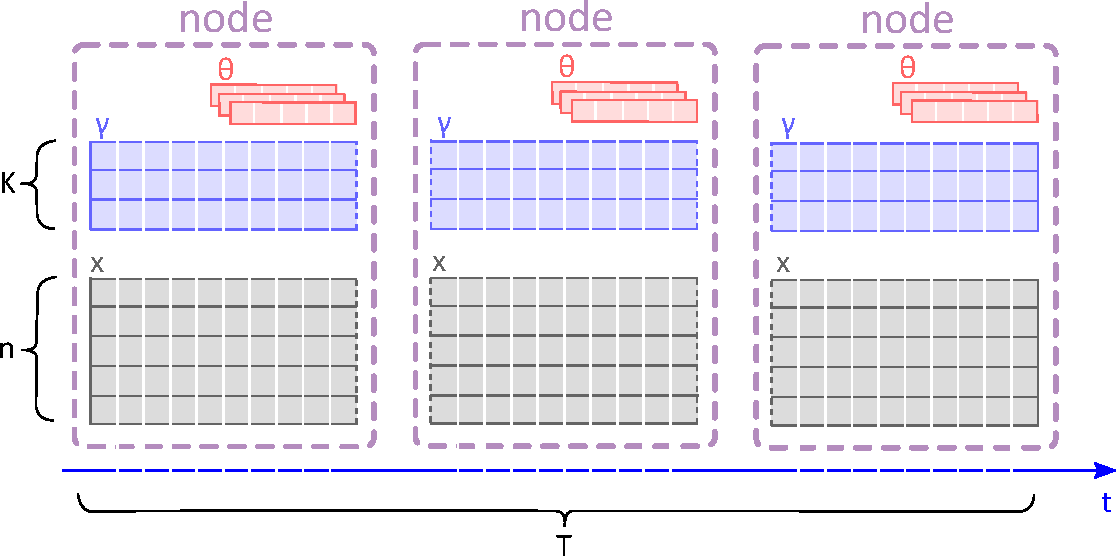
\includegraphics[width=0.50\linewidth, angle=0, clip = true]{figures/parallel.pdf}
			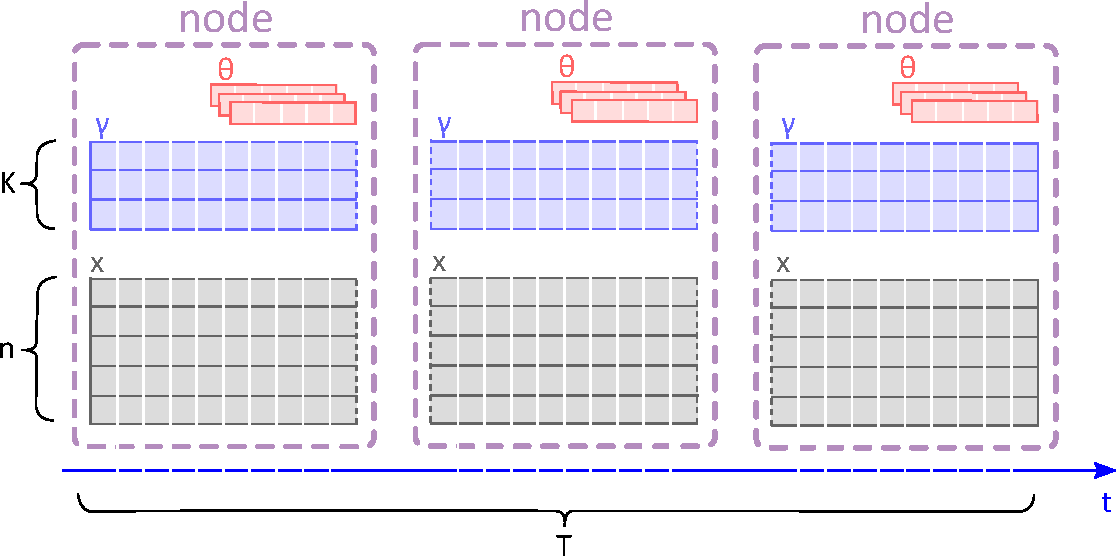
\includegraphics[width=0.50\linewidth, angle=0, clip = true]{figures/parallel.pdf}
			\caption{Computation on large-scale time-series data. We naturally split the data and indicator functions through the time-series. There are
			running several parallel jobs (computational units), which solve the problem with different initial conditions / number of clusters / integer model parameters.
					 }
			\label{fig:parallelisation}		 
		\end{center}
	\end{figure}
\end{column}	
\begin{column}{0.02\linewidth}\end{column}
\end{columns}

\vskip2ex

In furture work, we create a management on the top of this approach. Each computing unit will consist of the set of nodes operating together on one data vector solving
one particular problem of given $K$ and the set of random initial values of $\gamma$. 

Also this parallel time-series splitting layout brings naturally the idea of the domain decomposition methods for solving not only inner QP \label{eq:qp}, 
but also a whole original optimisation problem \eqref{eq:general}.

\end{block}

\begin{block}{Toy model: Geometrical time-dependent clustering with K-means model} 

Geometrical clustering problem represents the most basic modelling functions - constant function. 
We are trying to model the given data using the one value in every cluster in least-square sence
\begin{displaymath}
 \forall t \in T_k: x_t = \theta_k + \epsilon_t ~~~ 
 L(\theta_1, \dots, \theta_K, \Gamma) 
 = \sum\limits_{t = 0}^{T} \sum\limits_{k = 1}^{K} \gamma_k(t) \Vert x_t - \theta_k \Vert^2 ~~ \rightarrow \min 
\end{displaymath}

The early Matlab implementation revealed the main algorithm challenges, see Figure \ref{fig:kmeans_matlab}. The inner problems in Algorithm \ref{alg:outer} could reuse the solution from previous outer iteration
as an initial approximation in new solution process. Moreover, it is not necessary to solve problems exactly and adaptive precision control should be proposed and implemented.

\begin{columns}[T]
\begin{column}{0.02\linewidth}\end{column}
\begin{column}{0.94\linewidth}
	\begin{figure}[H]
		\begin{center}
			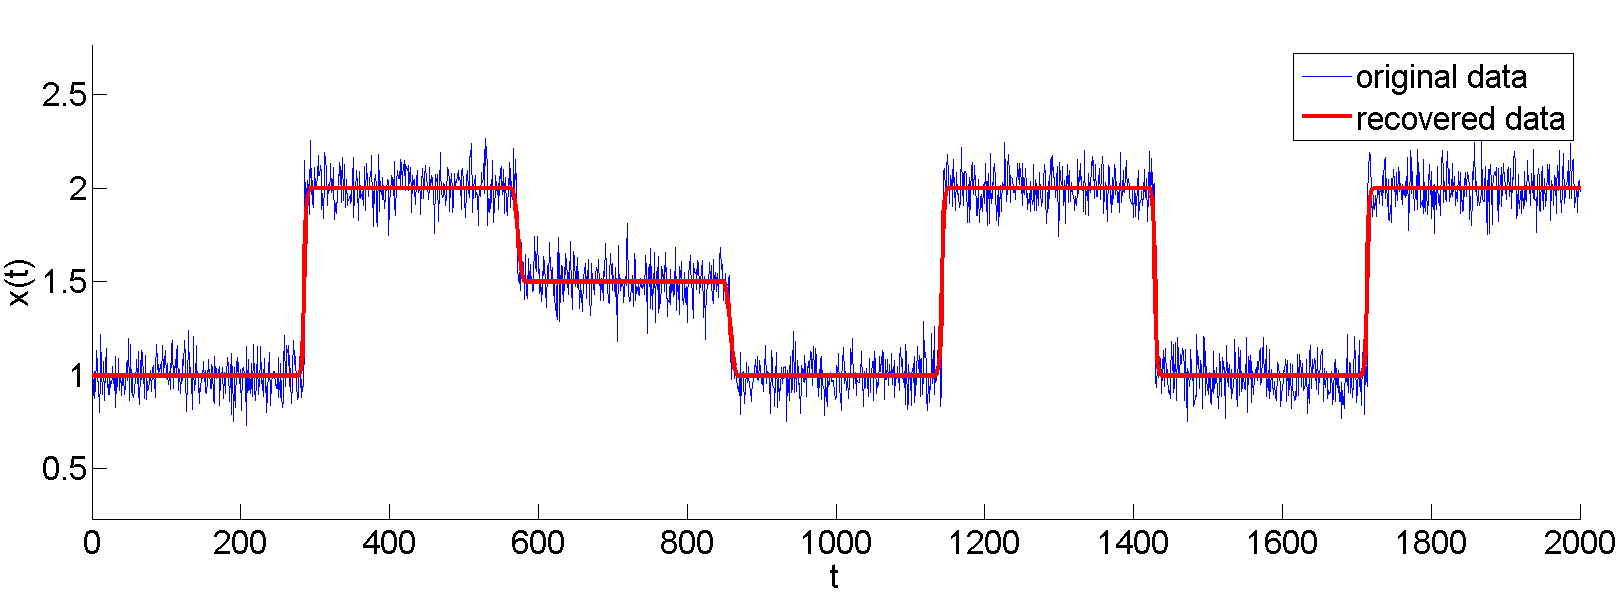
\includegraphics[width=0.49\linewidth, angle=0, clip = true]{figures/kmeans1.png}
			\hfil
			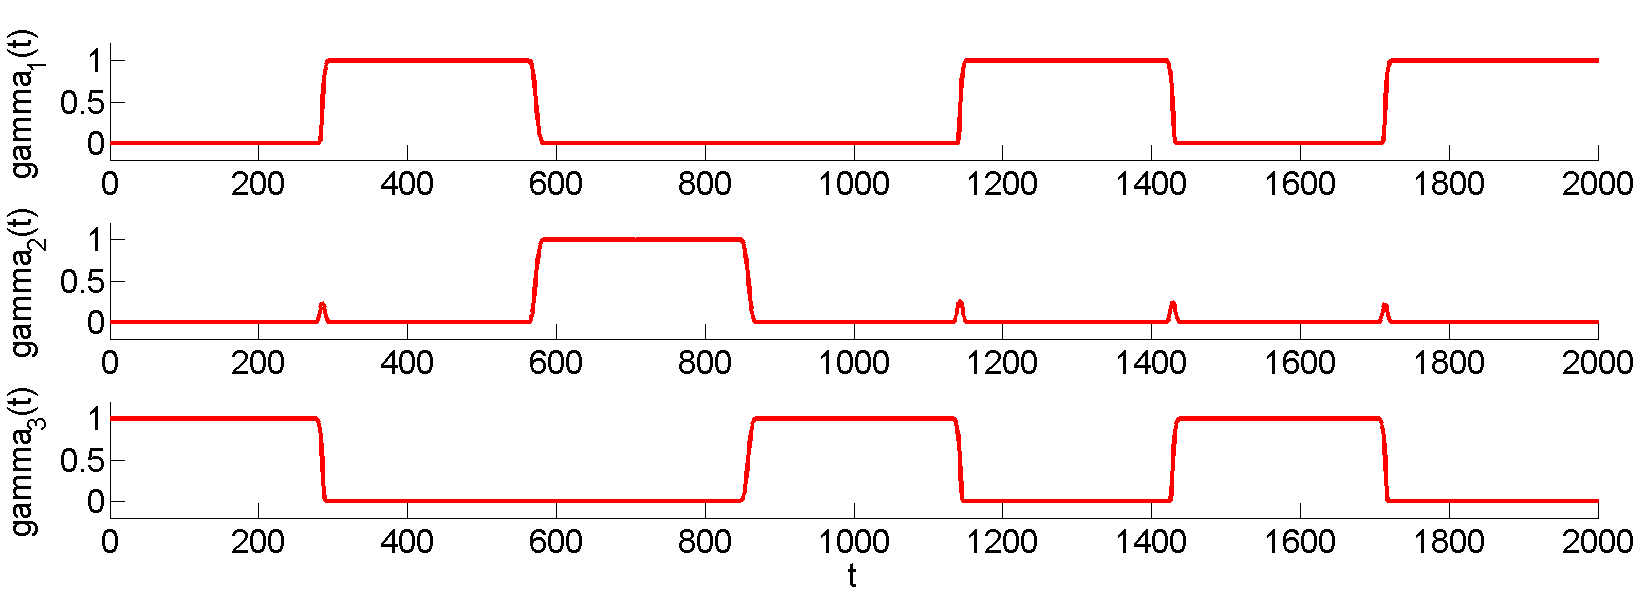
\includegraphics[width=0.49\linewidth, angle=0, clip = true]{figures/kmeans2.png}
			\caption{Initial example: one-dimensional K-means problem with $K=3, T=2000$ solved by FEM-BV-H1 in Matlab. The problem is solved in $4$ outer iterations, the inner QP problem (of dimension $K\cdot N = 6000$) is solved by Matlab \emph{quadprog} solver.
					 Let us remark that the Matlab implementation of \emph{'interior-point-convex'} algorithm is not able to use approximation of solution from previous outer iteration as an initial guess of the solution. Moreover, it is not able to control the precision based on the decrease of the objective function.
					 In projected gradient methods (like SPG-QP), we are able to control the decrease in every iteration as well as use initial approximation.
					 }
			\label{fig:kmeans_matlab}		
		\end{center}
	\end{figure}
\end{column}	
\begin{column}{0.02\linewidth}\end{column}
\end{columns}

\vskip2ex
We implement Algorithm \ref{alg:outer} and Algorithm \ref{alg:spg_qp} in PETSc framework and solve K-means problem on 2 nodes on PIZ Daint machine (Intel Xeon E5-2670 (8 cores, 32GB) with NVIDIA Tesla K20X (2688 cores, 6GB))
. The results are presented in Figures \ref{fig:kmeans_pizdaint1}, \ref{fig:kmeans_pizdaint3}, \ref{fig:indicator}, and \ref{fig:L}.
 
\begin{columns}[T]
\begin{column}{0.02\linewidth}\end{column}
\begin{column}{0.46\linewidth}
	\begin{figure}[H]
		\begin{center}
			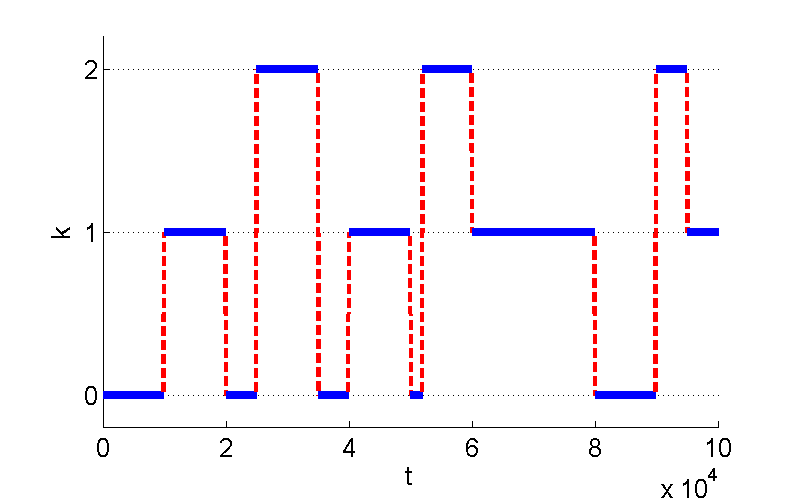
\includegraphics[width=1.0\linewidth, angle=0, clip = true]{figures/generator.png}
			\caption{Large-scaled example: Switching schema for generating testing benchmark.
					 }
			\label{fig:kmeans_pizdaint1}	
		\end{center}
	\end{figure}

	\begin{figure}[H]
		\begin{center}
			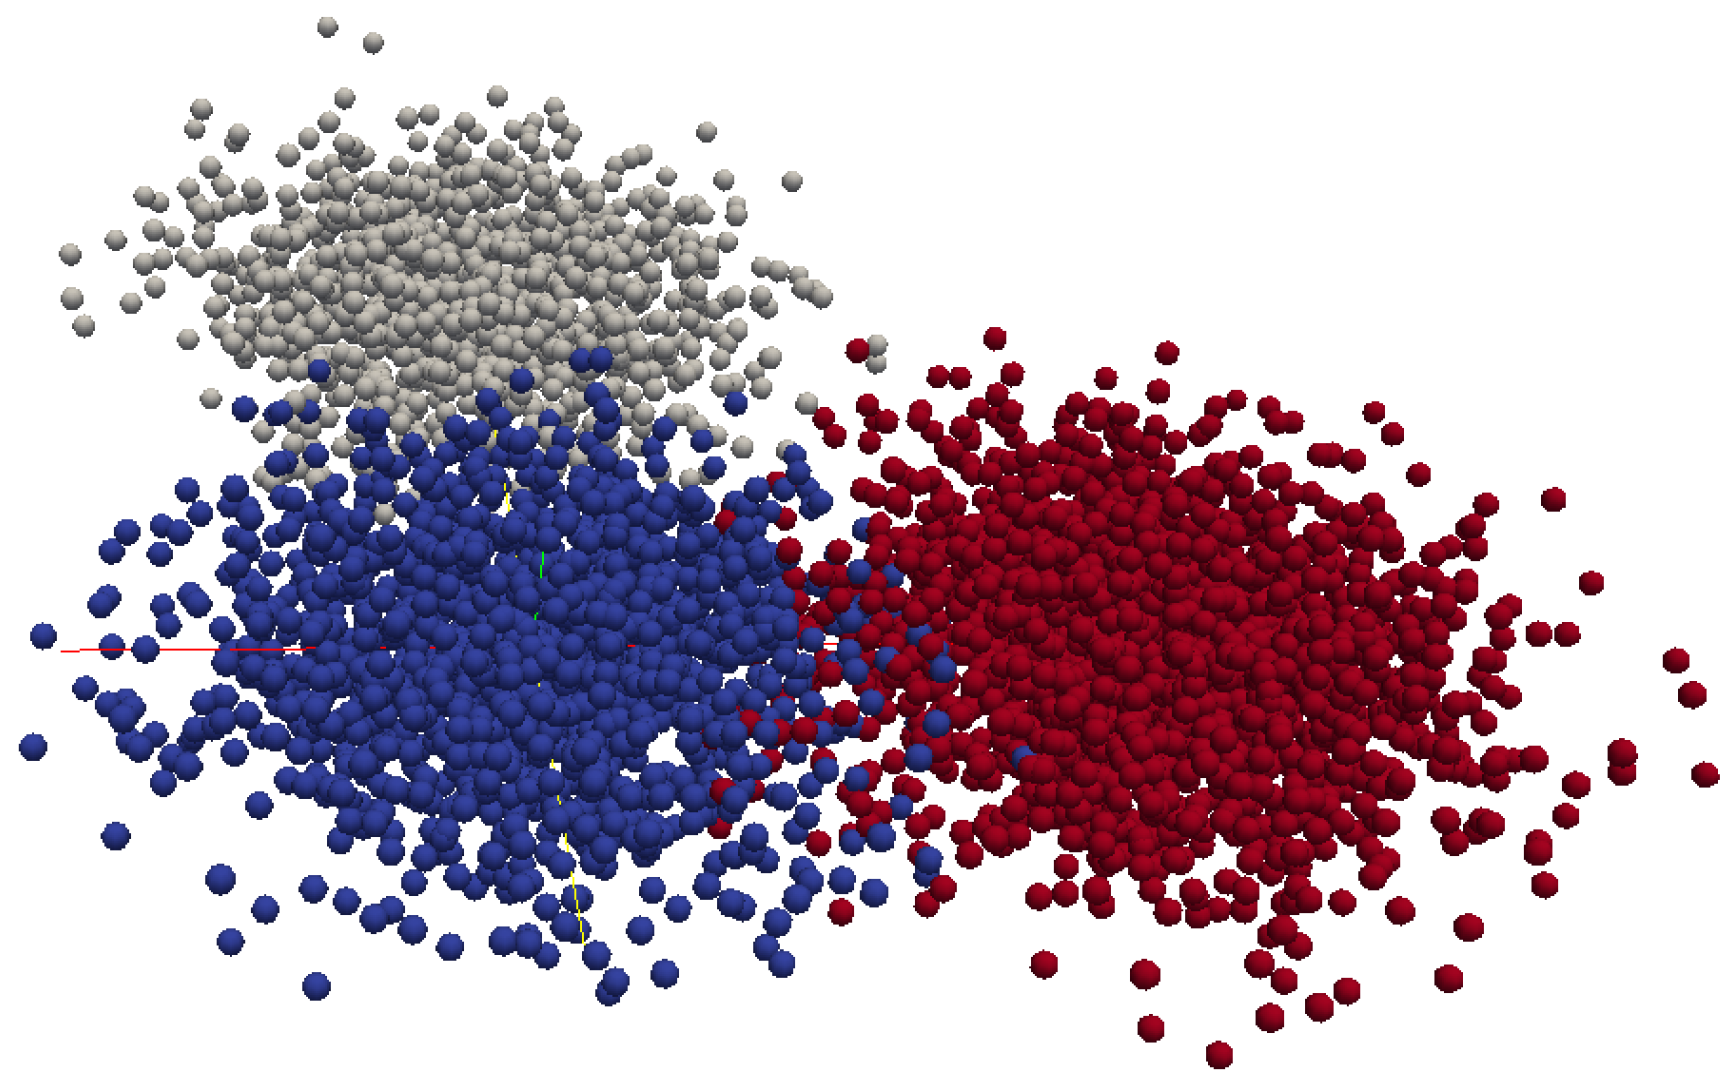
\includegraphics[width=1.0\linewidth, angle=0, clip = true]{figures/solution.png}
			\caption{The solution: clustered data. The affiliation to the cluster is decided by the maximum value of indicator functions $\gamma_0, \gamma_1, \gamma_2$ (see Figure \ref{fig:indicator}). For visualisation, we used VTK format openable in Paraview.
					 }
			\label{fig:kmeans_pizdaint3}	
		\end{center}
	\end{figure}
\end{column}	
\begin{column}{0.02\linewidth}\end{column}
\begin{column}{0.46\linewidth}
	\begin{figure}[H]
		\begin{center}
			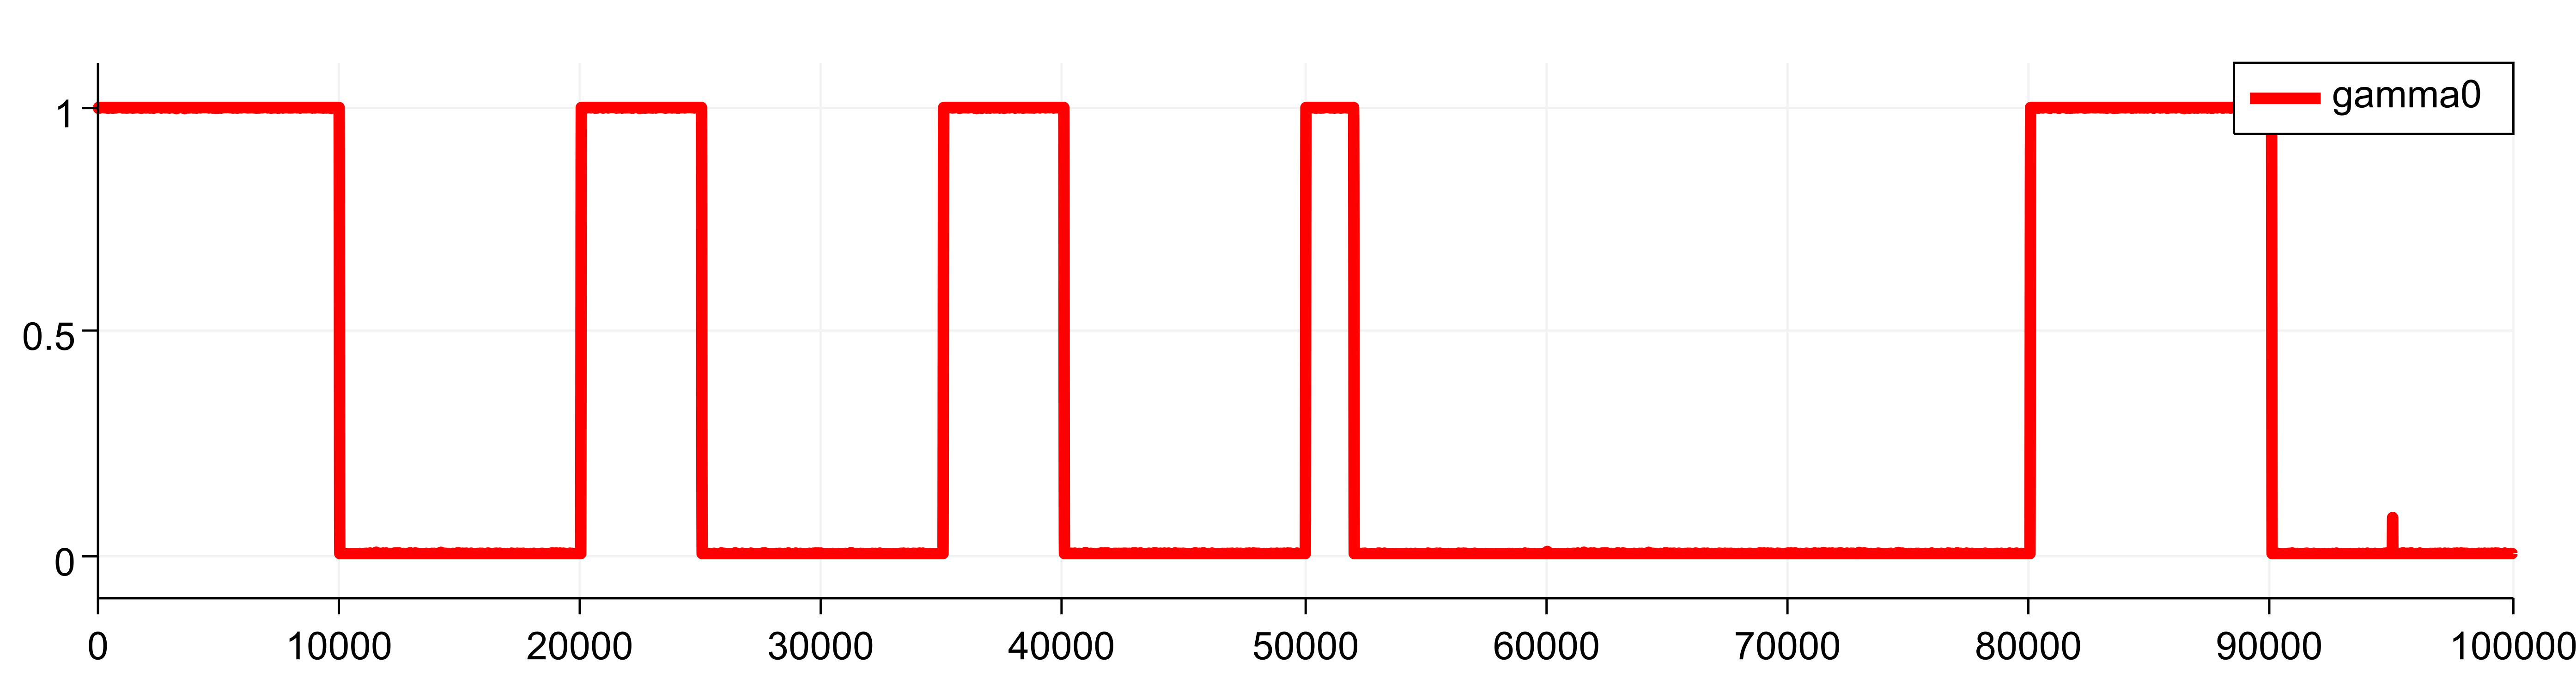
\includegraphics[width=1.0\linewidth, angle=0, clip = true]{figures/gamma0.png} \\
			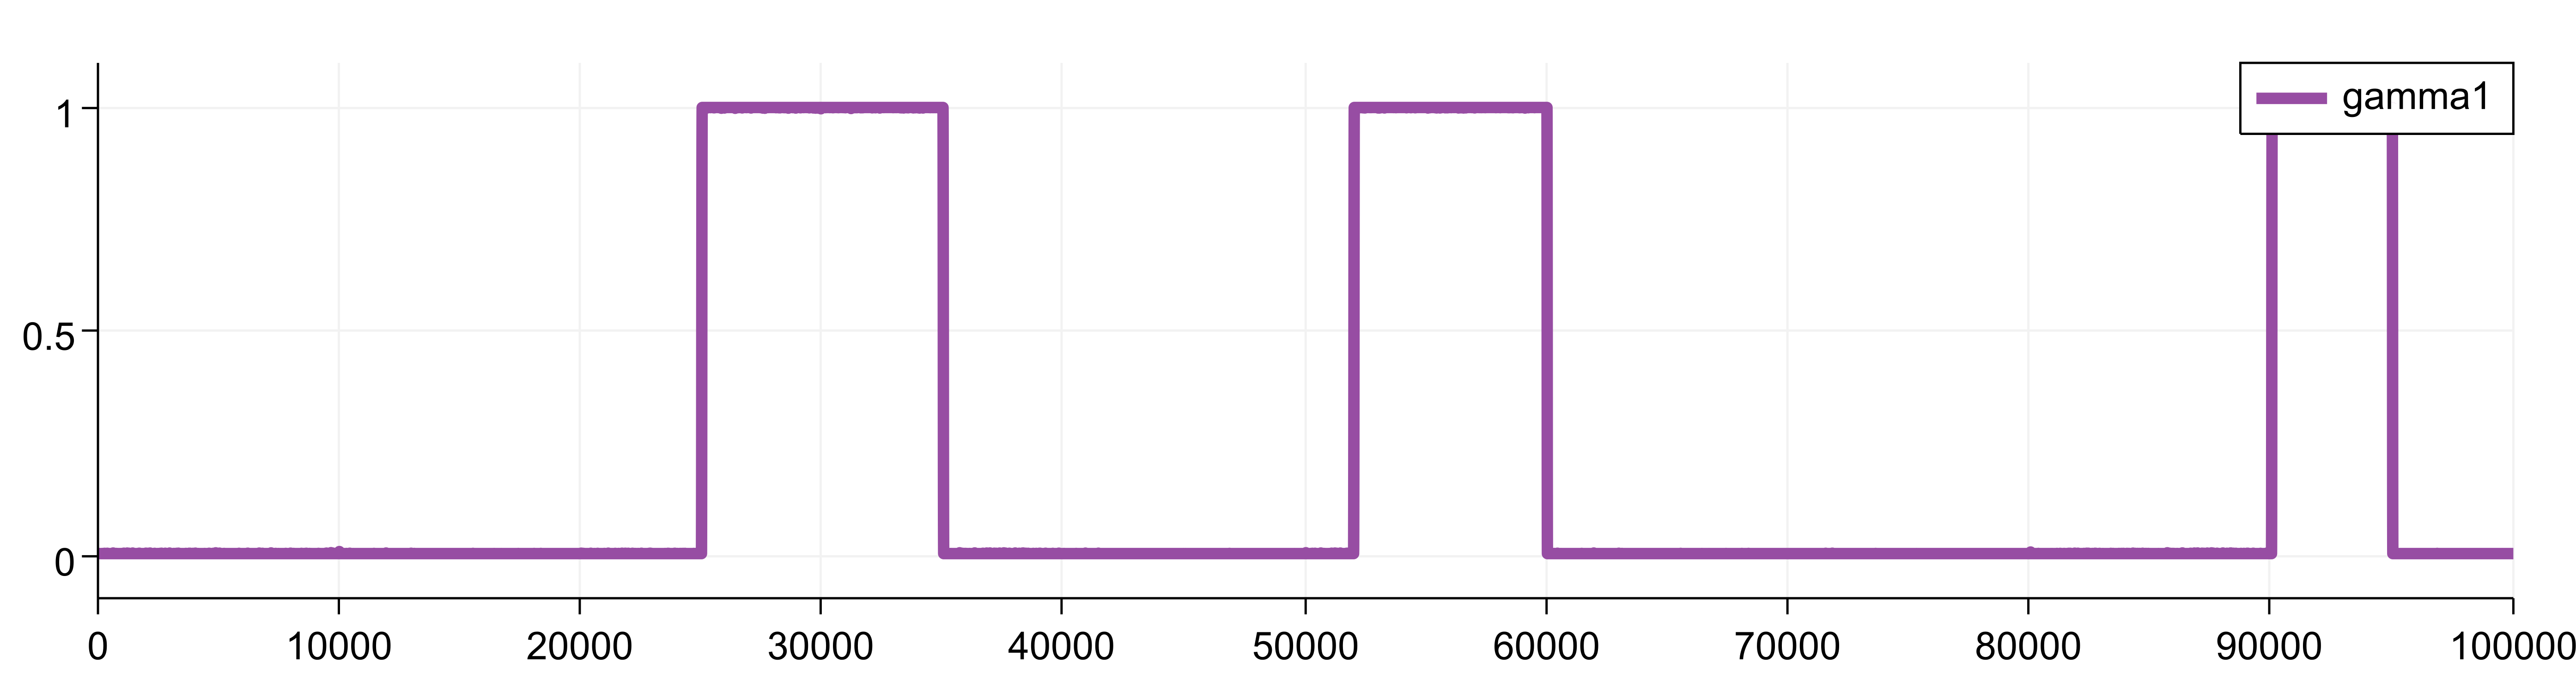
\includegraphics[width=1.0\linewidth, angle=0, clip = true]{figures/gamma1.png} \\
			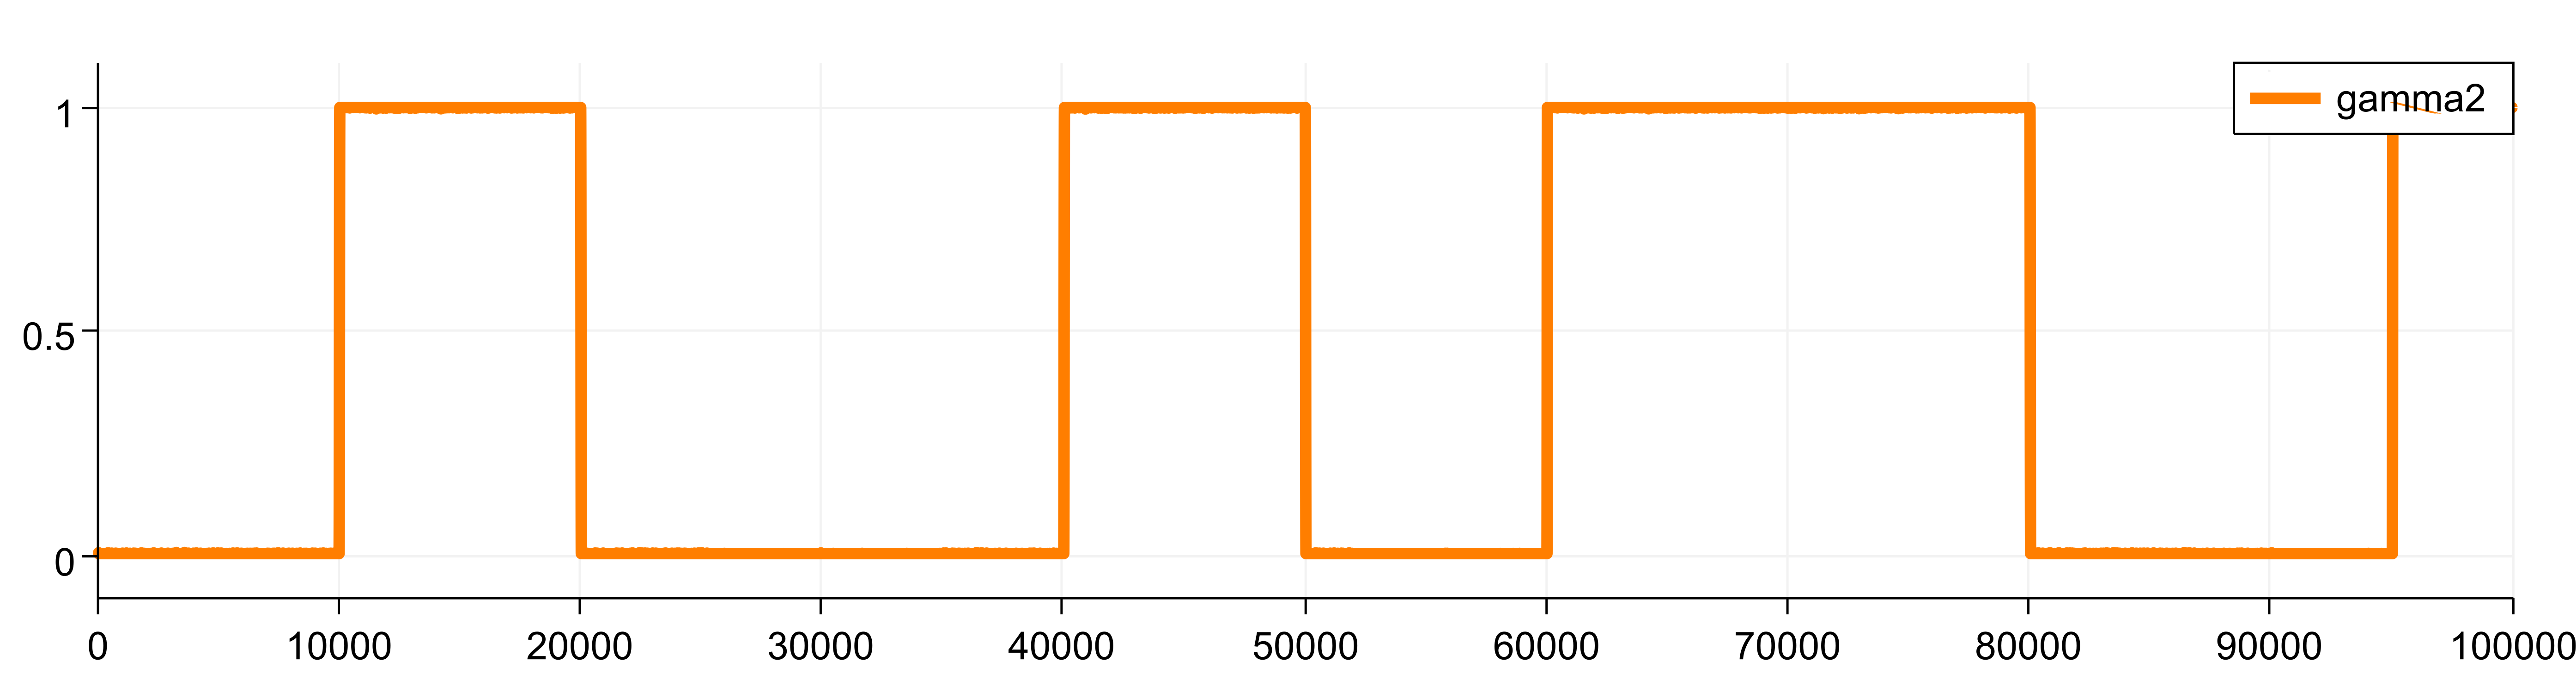
\includegraphics[width=1.0\linewidth, angle=0, clip = true]{figures/gamma2.png} 

			\caption{The solution: indicator model function in FEM-BV-H1 model found using our new library. 
					 Library generates files suitable for ParaView.
					 }
			\label{fig:indicator}	
		\end{center}
	\end{figure}
	\begin{figure}[H]
		\begin{center}
			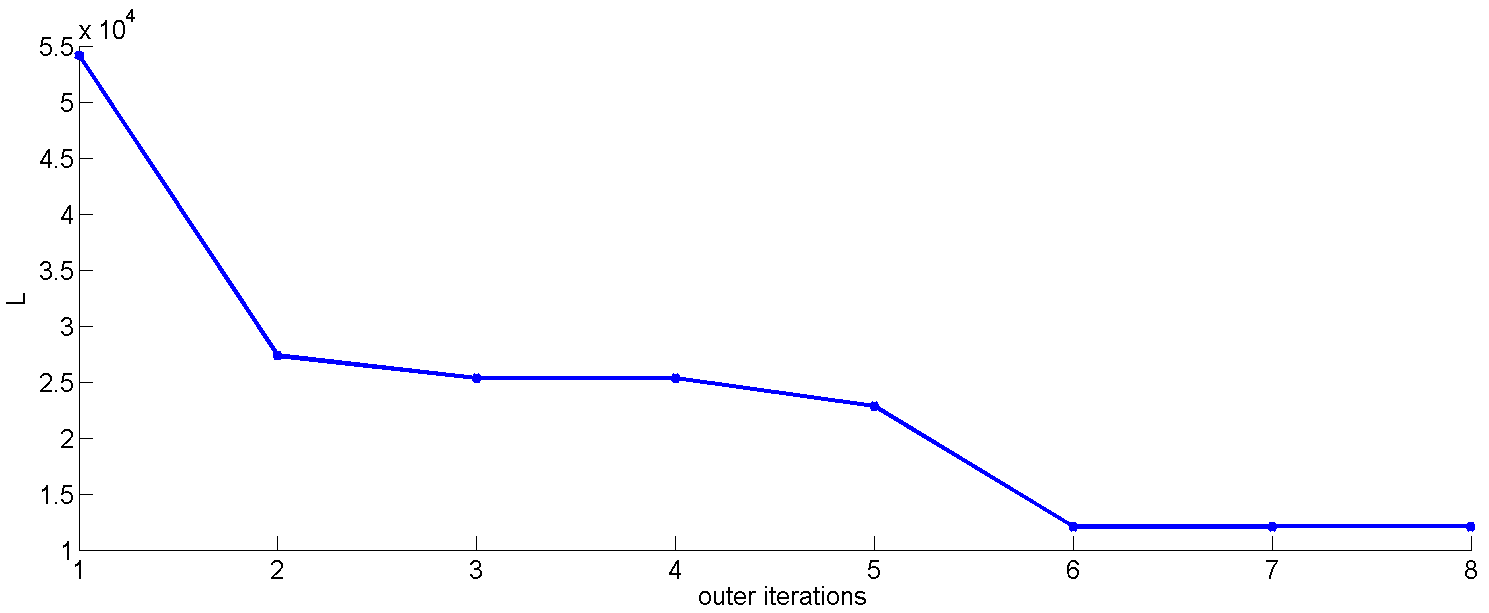
\includegraphics[width=1.0\linewidth, angle=0, clip = true]{figures/L.png} \\

			\caption{Monotone decrease of global objective function during outer iterations. Our algorithm is terminated when the difference of objective function is less than $10^{-4}$.
					 }
			\label{fig:L}	
		\end{center}
	\end{figure}
\end{column}	
\begin{column}{0.02\linewidth}\end{column}
\end{columns}





\end{block}

\begin{block}{Future work: from Time-Regularisation to Graph-Regularisation} 

\begin{columns}[T]
\begin{column}{0.02\linewidth}\end{column}
\begin{column}{0.66\linewidth}
	\begin{figure}[H]
		\begin{center}
			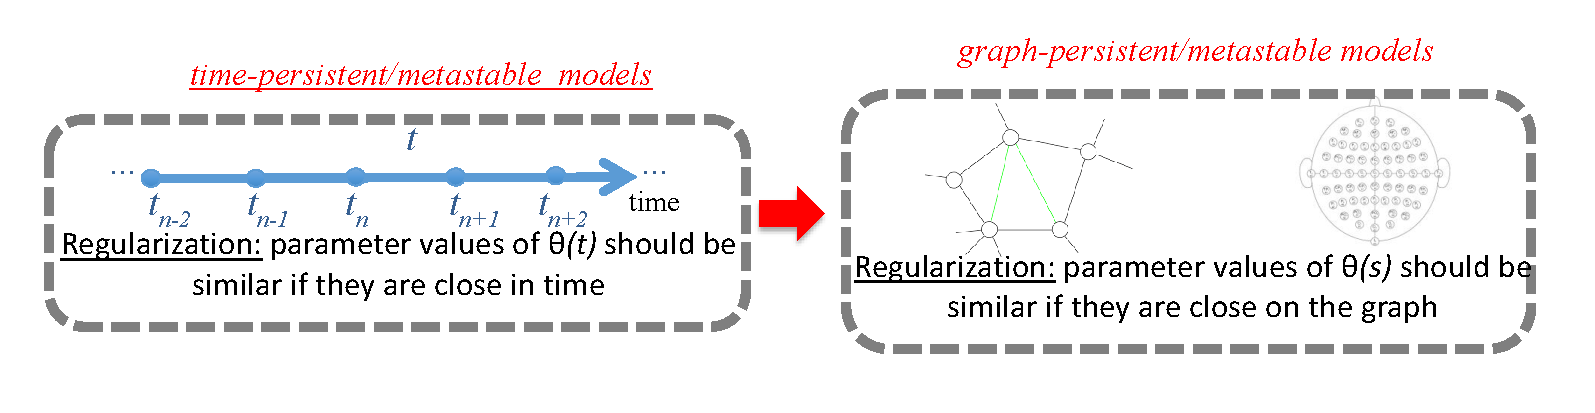
\includegraphics[width=1.0\linewidth, angle=0, clip = true]{figures/graph.pdf}
			\label{fig:graph}	
		\end{center}
	\end{figure}

 \begin{displaymath}
  \begin{array}{l}
  H = 2\textrm{diag} \left( \sum \vert W_{i,:} \vert \right) - 2 W, ~~~ W = G \circ B, ~~~ B = ~\textrm{3-diag} (1,1,1) \\
  G - ~\textrm{graph connectivity matrix}, ~~~ \circ - ~\textrm{Kronecker product}
  \end{array}
 \end{displaymath}
 \vskip2ex
 Matrix-vector multiplication still can be written in matrix-free form and effectivelly performed on GPU. Moreover, the constraints of the QP problem remain the same, therefore the projection problem could be solved in full-parallel way.
\end{column}	
\begin{column}{0.02\linewidth}\end{column}
\begin{column}{0.26\linewidth}
	\begin{figure}[H]
		\begin{center}
			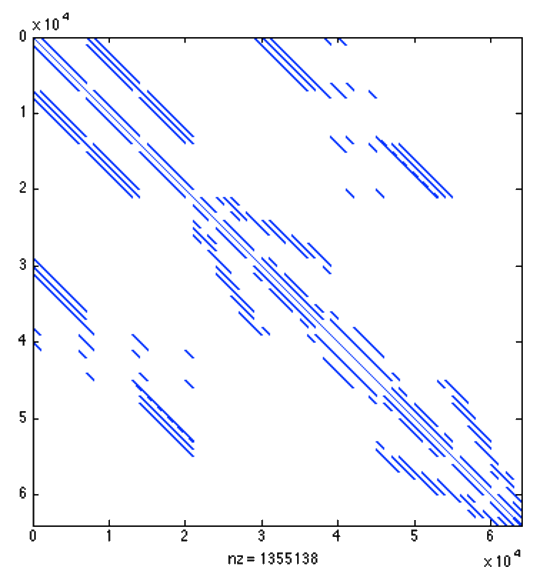
\includegraphics[width=1.0\linewidth, angle=0, clip = true]{figures/matrix.png} \\
			\caption{Example: pattern of Hessian matrix in Graph-regularisation.}
			\label{fig:L}	
		\end{center}
	\end{figure}
\end{column}	
\begin{column}{0.02\linewidth}\end{column}
\end{columns}


\end{block}




%----------------------------------------------------------------------------------------
%	REFERENCES
%----------------------------------------------------------------------------------------

\begin{block}{References}
        
\nocite{*} % Insert publications even if they are not cited in the poster
\small{

\bibliography{ams}
\bibliographystyle{apalike}
%\bibliographystyle{unsrt}

%% BIBLIOGRAPHY 
\begin{thebibliography}{}

\bibitem{brockwell2002}
P.~Brockwell and R.~Davis.
{\em Introduction to Time Series and Forecasting}.
Springer, Berlin, 2002.

\bibitem{granger69}
C.~Granger.
{\em Investigating causal relations by econometric models and cross-spectral methods}.
Econometrica, 37:424--438, 1969.

\bibitem{horenko_fem}
I.~Horenko.
{\em Finite Element Approach to Clustering of Multidimensional Time Series}.
SIAM J. Sci. Comp. 32, 62--83, 2010.

\bibitem{horenko_pnas_2014}
S.~Gerber and I.~Horenko.
{\em On inference of causality for discrete state models in a multiscale context}.
Proc. Natl. Acad. Sci. USA (PNAS), 2014.

\bibitem{horenko_aaas_2015}
S.~Gerber and I.~Horenko.
{\em Improving Clustering by Imposing Network Information}.
Sciences Advances (AAAS), 1(7):e1500163, 2015


\bibitem{metzner_2012}
P.~Metzner, L.~Putzig, and I.~Horenko.
{\em Analysis of persistent non-stationary time series and applications}.
 CAMCoS 7, 175--229, 2012.

\bibitem{pospisil_phd}
L.~Pospisil.
{\em Development of Algorithms for Solving Minimizing Problems
with Convex Quadratic Function on Special Convex Sets and Applications}.
PhD thesis, supervised by Z.~Dostal, VSB-TU Ostrava, 2014.

\bibitem{spg}
E.G.~Birgin, J.M~Martinez, and M.M.~Raydan.
{\em Nonmonotone spectral projected gradient methods on convex sets}. 
SIAM Journal on Optimization 10, 1196--1211, 2000.

\bibitem{simplex}
Y.~Chen, X.~Ye.
{\em Projection Onto A Simplex}.
Arxiv. 1101.6081, 2012.


\end{thebibliography}

}

\end{block}




%----------------------------------------------------------------------------------------

\end{column} % End of the second column

\begin{column}{.008\textwidth}\end{column} % Empty spacer column

\end{columns} % End of all the columns in the poster

\end{frame} % End of the enclosing frame

\end{document}
